\section{Introduction}
\label{sec:intro}
Data stream clustering (\dsc) is a crucial operation in data stream mining, with applications in network intrusion detection~\cite{KDD99}, social network analysis~\cite{EDMStream:17}, weather forecasting~\cite{weather_forecast:2020}, and financial market analysis~\cite{cai2012clustering}. Unlike traditional batch clustering algorithms such as \kmeans~\cite{KMeans:1967,KMeans:1982} and \dbscan~\cite{DBSCAN:1996}, \dsc algorithms dynamically group incoming data based on attribute similarities and adjust clustering results upon receiving the new streaming data. \dsc algorithms must be efficient~\cite{EmpiricalR:2017,Empirical:2018}, as they are used in high-velocity environments requiring real-time decisions. Additionally, these algorithms need to address unique challenges in data stream scenarios, such as \emph{cluster evolution} and \emph{outlier evolution}~\cite{EDMStream:17,concept_evolution:2010,Concept_Evolution:10,Concept_Evolution:16,Concept_Drift_Survey:2018}, which involve the changing distribution of data and the emergence of new outliers over time and the changing dimensions of data points.

The diverse applications and performance requirements of \dsc have led to the development of numerous \dsc algorithms~\cite{BIRCH:96,Clustream:03,EDMStream:17,DenStream:06,DBStream:16,DStream:2007,SL-KMeans:20,StreamKM++:12,TSFDBSCAN:20,DenStream:06,Stream_Clustering_Survey01,Survey13}. \emph{However, these algorithms, while effective to varying extents, often lack the flexibility and self-optimization capabilities needed to adapt to diverse application contexts.} Typically, \dsc algorithms consist of four main components~\cite{wang2023sesame}: the summarizing data structure, the window model, the outlier detection mechanism, and the refinement strategy. Design choices in each component vary to meet specific needs based on application requirements, data characteristics, or performance objectives. For instance, some algorithms are optimized for processing speed~\cite{DStream:2007}, making them ideal for high-velocity data streams, while others prioritize clustering accuracy~\cite{StreamKM++:12,BIRCH:96}, a critical factor in applications requiring precise cluster assignments. The task of selecting an appropriate \dsc algorithm for real-world, diverse workloads becomes complex due to the interdependent nature of these design choices, each with its own set of trade-offs and performance implications~\cite{wang2023sesame}.


\begin{figure}[t]
	\centering
	\begin{minipage}{1\linewidth}
        \centering
		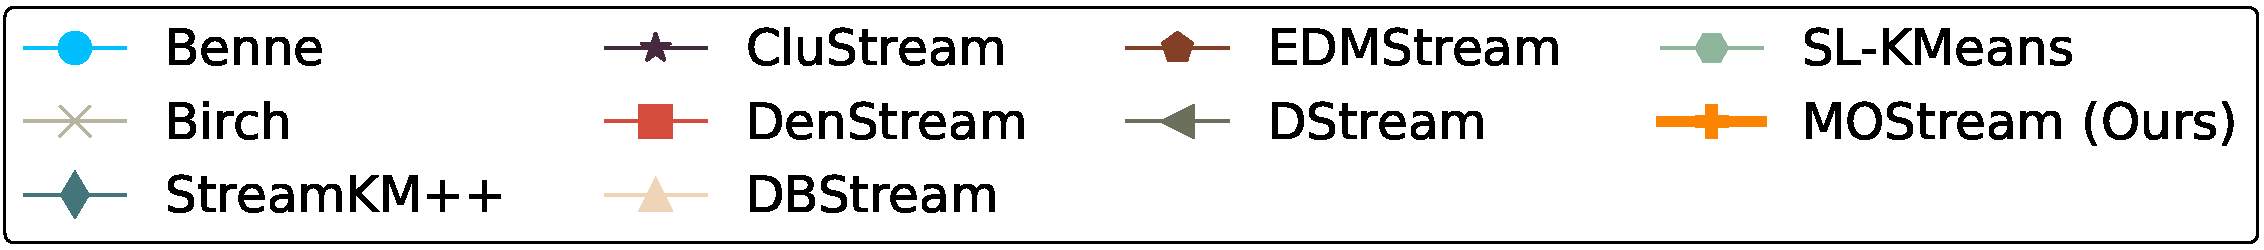
\includegraphics[width=1\linewidth]{Figures/Experiment/Motivation/Motivation_Legend.pdf}		
	\end{minipage}
	\begin{subfigure}{.245\textwidth}
        \centering
        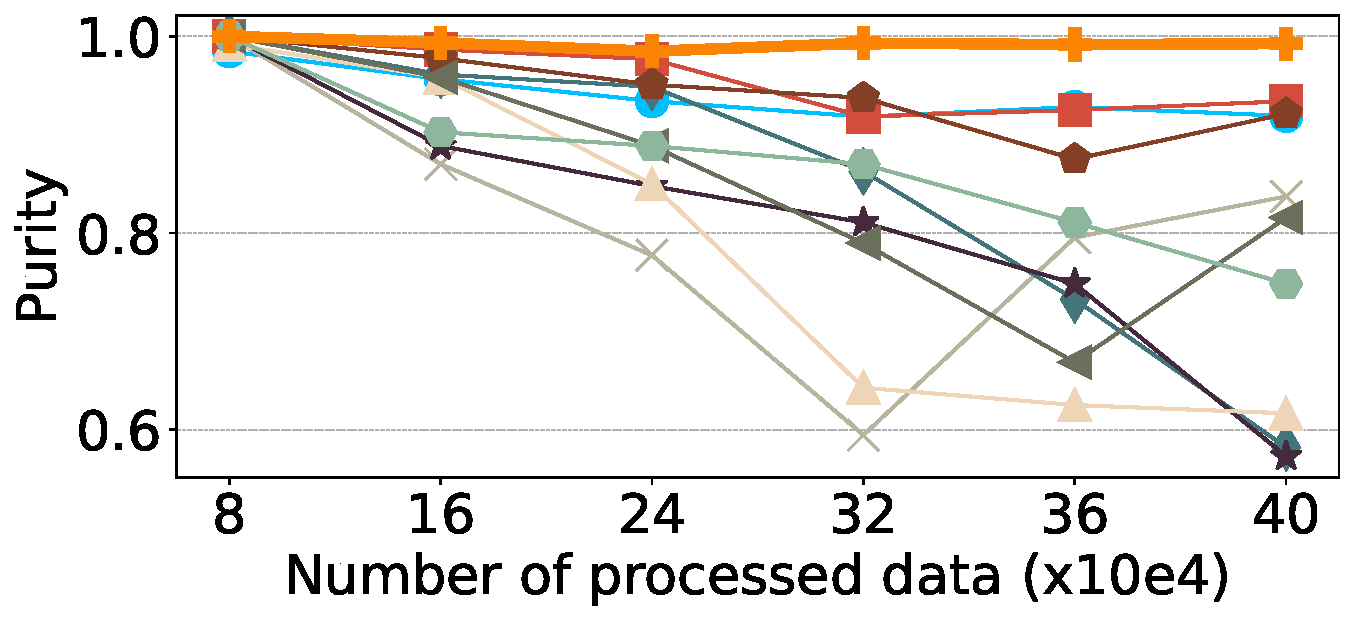
\includegraphics[width=\linewidth]{Figures/Experiment/Motivation/Motivation_Purity.pdf}      
         \caption{Accuracy}
         \label{fig:moti_purity}
	\end{subfigure}       
  	\begin{subfigure}{.235\textwidth}
        \centering
        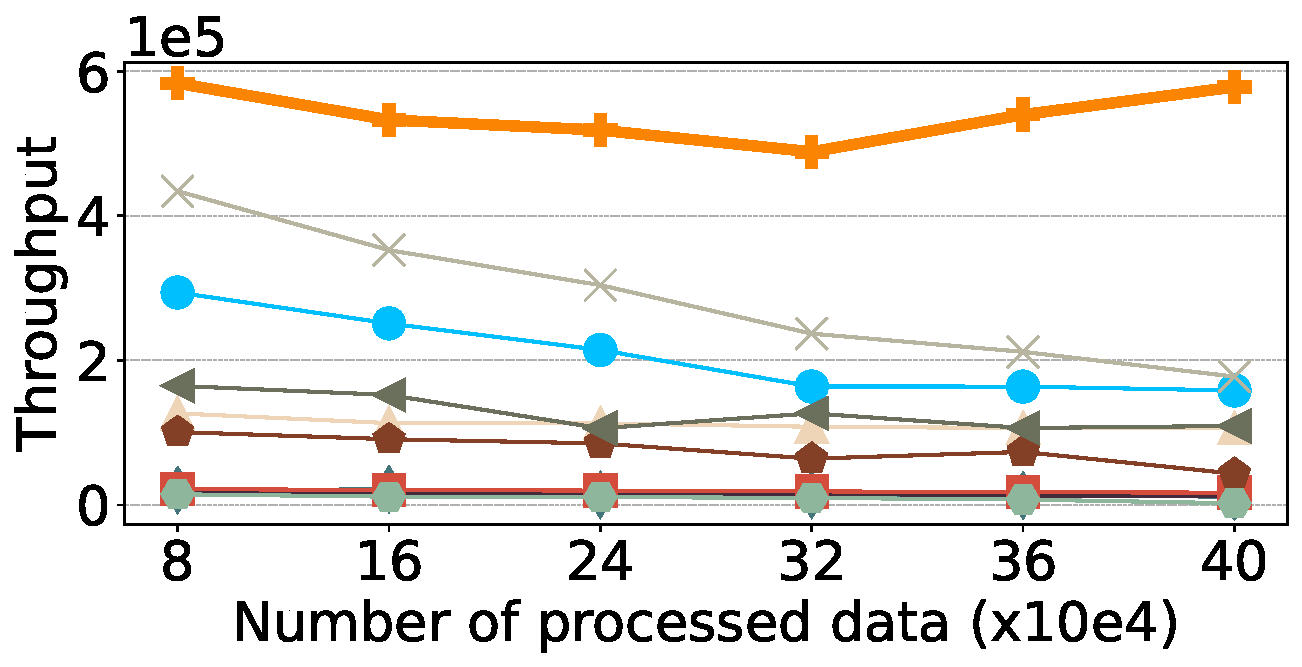
\includegraphics[width=\linewidth]{Figures/Experiment/Motivation/Motivation_Throughput.pdf}
        \caption{Efficiency}
        \label{fig:moti_throughput}
	\end{subfigure}     
        \caption{Performance comparison of nine representative \dsc algorithms and \algo on \kdd with high frequency of outlier evolution and increasing frequency of cluster evolution in the dataset.}
\label{fig:motivation}
\end{figure}


% \begin{figure}[t]
% \centering
% % \includegraphics[width=0.5\textwidth]{performance_comparison.png}
% \caption{Performance comparison of 9 representative \dsc algorithms on dynamic workloads with increasing frequency of outlier evolution.}
% \label{fig:motivation}
% \end{figure}

Figure~\ref{fig:motivation} shows the performance comparison of nine representative \dsc algorithms, including \benne~\cite{wang2023sesame}, \birch~\cite{BIRCH:96}, \skm~\cite{StreamKM++:12}, \clustream~\cite{Clustream:03}, \denstream~\cite{DenStream:06}, \dbstream~\cite{DBStream:16}, \edmstream~\cite{EDMStream:17}, \dstream~\cite{DStream:2007}, and \slkmeans~\cite{SL-KMeans:20} and our proposed algorithm \algo on \kdd with high frequency of outlier evolution and increasing frequency of cluster evolution in the dataset. We observe that both the accuracy and efficiency of existing algorithms suffer from severe degradation when processing more and more streaming data with high frequency of outlier evolution. We attribute this degradation to the inability of their static design choices to dynamically adapt to workload evolution. \benne, for example, allows manual selection of different design options for each of the four design aspects of a \dsc algorithm. While it provides a flexible framework for exploring design choices, it requires manual intervention to select the optimal configuration, which may not be practical in dynamic and rapidly changing data stream environments. In contrast, \algo\footnote{Code is at \url{https://github.com/intellistream/Sesame}} achieves highest accuracy and efficiency during the entire clustering process due to its modular and self-optimizing feature that adapts to changing workload characteristics with little overhead.

% \textbf{Novelty and Contribution.}
Similar to \benne, \algo adopts a \textbf{modular} architecture that allows flexible choices at each design aspect of \dsc algorithms and conducts a  dynamic adjustment of the modular architecture for adapting to the new worload characteristics. By further integrating dynamic adaptability, comprehensive component selection, and novel adaptation techniques, \algo effectively addresses the inherent challenges of \dsc through \textbf{self-optimizing}:
% It further achieves significant improvements over the state-of-the-art by following key innovations:

\emph{1. Dynamic Adaptability:} Unlike \benne, which uses a fixed modular configuration, \algo dynamically detects changes in workload characteristics and reconfigures itself in real-time. This capability allows \algo to maintain optimal performance under varying data stream conditions, effectively managing issues such as sudden changes in data dimensionality and outlier frequency.

\emph{2. Comprehensive Component Selection:} \algo includes an automated selection mechanism that not only considers individual component optimization but also evaluates the interplay between different design aspects (summarizing data structure, window model, outlier detection, and refinement strategy). This holistic approach ensures that the algorithm can adapt more comprehensively to diverse data stream scenarios compared to existing methods.

\emph{3. Novel Techniques for Adaptation:} \algo introduces novel techniques for flexible migration and regular stream characteristics detection, which are crucial for maintaining high performance in dynamic environments. These techniques are not present in existing algorithms like \benne and significantly enhance \algo's adaptability and efficiency.

\emph{4. Extensive Empirical Evaluations:} Through extensive empirical evaluations, \algo demonstrates superior performance in both accuracy and efficiency metrics across a wider range of datasets, including real-world and synthetic datasets with evolving characteristics. In-depth studies are also conducted to better comprehend \algo's dynamic composition capability. This breadth of evaluation underscores \algo's robustness and versatility.

Comprehensive analysis and rigorous performance evaluation with 9 representative \dsc algorithms on 4 real-world datasets and 3 synthetic datasets show that \algo consistently surpasses competing algorithms in clustering accuracy, processing throughput, and adaptability to varying data stream characteristics, including varying cluster evolution, outlier evolution, and workload dimensionality. 
% Our evaluation, spanning a wide range of real-world and synthetic workloads, validates \algo's effectiveness and generalizability. 
% Notably, \algo demonstrates superior performance in purity, CMM, and throughput metrics, particularly in scenarios characterized by high dimensionality and frequent cluster evolution.

The rest of the paper is organised as follows: Section~\ref{sec:background} introduces the background of \dsc algorithms. Section~\ref{sec:algorithm_design} discusses the algorithmic design of \algo. Section~\ref{sec:evaluation} presents our empirical evaluation of \algo. Finally, Section~\ref{sec:relatedwork} reviews additional related work, and Section~\ref{sec:conclusion} concludes the paper.